\documentclass[11pt,letterpaper]{article}
\usepackage[margin=2.5cm,top=3.5cm,bottom=3cm]{geometry}
\usepackage{booktabs}
\usepackage{graphicx}
\usepackage[hidelinks]{hyperref}
\usepackage{microtype}
\usepackage[table,dvipsnames]{xcolor}
\usepackage{longtable}
\usepackage{array}
\usepackage{caption}
\usepackage[T1]{fontenc}
\usepackage{lmodern}
\usepackage{fancyhdr}
\usepackage{amsmath}
\usepackage{titlesec}
\usepackage{enumitem}

\definecolor{wavblue}{RGB}{26,58,92}
\definecolor{wavgray}{RGB}{120,120,120}
\definecolor{wavlight}{RGB}{235,242,250}
\definecolor{wincolor}{RGB}{0,110,0}

\graphicspath{{/Users/egs/repos/waverider/benchmarks/canonical_tests/}}

\pagestyle{fancy}
\fancyhf{}
\fancyhead[L]{\small\color{wavgray}Manifold-Informed Architecture Benchmark \textemdash\ HEART}
\fancyhead[R]{\small\color{wavgray}\texttt{waverider @ 054030a}}
\fancyfoot[C]{\small\color{wavgray}\thepage}
\renewcommand{\headrulewidth}{0.4pt}

\titleformat{\section}{\large\bfseries\color{wavblue}}{}{0em}{}[\color{wavblue}\titlerule]
\titleformat{\subsection}{\normalsize\bfseries\color{wavblue}}{}{0em}{}
\setlength{\parindent}{0pt}
\setlength{\parskip}{4pt plus 1pt}

\begin{document}

\begin{center}
  {\LARGE\bfseries\color{wavblue} Manifold-Informed Architecture Benchmark}\\[6pt]
  {\large HEART: 2 classes, 13D input}\\[8pt]
  {\small Generated: 2026-04-15 09:41:12 \quad$|$\quad Apple M5 Max MacBook Pro, 64 GB RAM, 2TB SSD}\\[2pt]
  {\small\texttt{waverider @ 054030a} (--abbrev-re
054030a600978c0e9ffac58faf7157939927d009) \quad$|$\quad 2026-04-14 22:20:05 -0400}
\end{center}
{\color{wavblue}\noindent\rule{\linewidth}{1.5pt}}
\medskip

\noindent\colorbox{wavlight}{\parbox{\dimexpr\linewidth-2\fboxsep\relax}{
  \smallskip
  \textbf{Best:} ManifoldModel ($\tau$=0.9)\quad test acc $= 0.8382 \pm 0.0247$\\[2pt]
  \textbf{vs Standard:} $+0.0286$ (2.86\,pp)\quad inf$\times$ fewer params\quad nan$\times$ acc/Kparam\\[2pt]
  \textbf{Manifold:} 13D $\rightarrow$ 9D (30.8\%\ noise dimensions)\\[2pt]
  \smallskip
}}
\bigskip

\section{Experimental Setup}

\begin{tabular}{@{}ll@{}}
\toprule
\textbf{Parameter} & \textbf{Value} \\
\midrule
  Dataset & HEART \\
  Input dimensionality & 13D \\
  Classes & 2 \\
  Intrinsic dim ($d$) & 9 \\
  Variance threshold ($\tau$) & 0.9 \\
  Epochs & 50 \\
  Trials & 3 \\
  Batch size & 32 \\
  Learning rate & 0.001 \\
  $k$ neighbors (local PCA) & 40 \\
\bottomrule
\end{tabular}

\section{Manifold Discovery}

Local PCA over the training set, $k = 40$ neighbors. Intrinsic dimensionality $d$ is taken as the maximum per-class maximum at $\tau = 0.9$, clamped to $n_{\mathrm{classes}} = 2$.

\begin{tabular}{@{}rrrrrr@{}}
\toprule
$\tau$ & Mean $d$ & Std & Min & Max & Noise (\%) \\
\midrule
  0.95 & 9.8 & 0.7 & 8 & 11 & 24.3 \\
  0.90 & 8.3 & 0.6 & 7 & 10 & 35.9 \\
  0.85 & 7.2 & 0.6 & 6 & 8 & 44.3 \\
  0.80 & 6.4 & 0.6 & 5 & 7 & 50.9 \\
\bottomrule
\end{tabular}

\subsection{Per-Class Intrinsic Dimensionality}

\begin{tabular}{@{}lrrrr@{}}
\toprule
Class & Mean $d$ & Std & Min & Max \\
\midrule
  1 & 8.6 & 0.5 & 8 & 9 \\
  0 & 8.1 & 0.7 & 7 & 9 \\
\bottomrule
\end{tabular}

\section{Architecture Comparison}

{\small
\begin{tabular}{@{}p{7cm}rccr@{}}
\toprule
\textbf{Architecture} & \textbf{Params} & \textbf{Test Acc ($\mu \pm \sigma$)} & \textbf{Loss} & \textbf{Acc/Kparam} \\
\midrule
  {Euclidean KNN (k=7)} & 0 & $0.8216 \pm 0.0205$ & --- & --- \\
  {\color{wincolor}ManifoldModel ($\tau$=0.9)\,$\star$} & 0 & $0.8382 \pm 0.0247$ & --- & --- \\
  {Standard (104$\rightarrow$52)} & 7,022 & $0.8096 \pm 0.0291$ & 0.6827 & 0.1153 \\
  {Manifold (2d$\rightarrow$d, d=9)} & 146 & $0.8064 \pm 0.0359$ & 0.4295 & 5.5231 \\
  {Wide Manifold (d+1=10)} & 162 & $0.8227 \pm 0.0401$ & 0.4103 & 5.0785 \\
  {Manifold+ManifoldAdam (d=9)} & 146 & $0.8152 \pm 0.0436$ & 0.4036 & 5.5836 \\
  {PCA$\rightarrow$9D + MLP (2d$\rightarrow$d)} & 371 & $0.8316 \pm 0.0331$ & 0.4102 & 2.2414 \\
  {Intrinsic Dim (PCA$\rightarrow$9D$\rightarrow$C)} & 110 & $0.8271 \pm 0.0393$ & 0.4055 & 7.5191 \\
\bottomrule
\end{tabular}
}

\smallskip
{\small $\star$ = best performing architecture}

\section{Key Findings}

\begin{itemize}[leftmargin=*,itemsep=3pt]
  \item \textbf{Best architecture:} ManifoldModel ($\tau$=0.9) \textemdash\ test accuracy $0.8382 \pm 0.0247$
  \item \textbf{vs Standard:} $+0.0286$ (2.86\,pp) accuracy gain
  \item \textbf{Parameter reduction:} inf$\times$ fewer parameters (0 vs 7,022)
  \item \textbf{Parameter efficiency:} nan$\times$ improvement (nan vs 0.1153 acc/Kparam)
  \item \textbf{Manifold compression:} 13D $\rightarrow$ 9D (30.8\%\ of ambient dimensions carry no structure)
\end{itemize}

\clearpage
\section{Result Figure}

\begin{figure}[htbp]
\centering
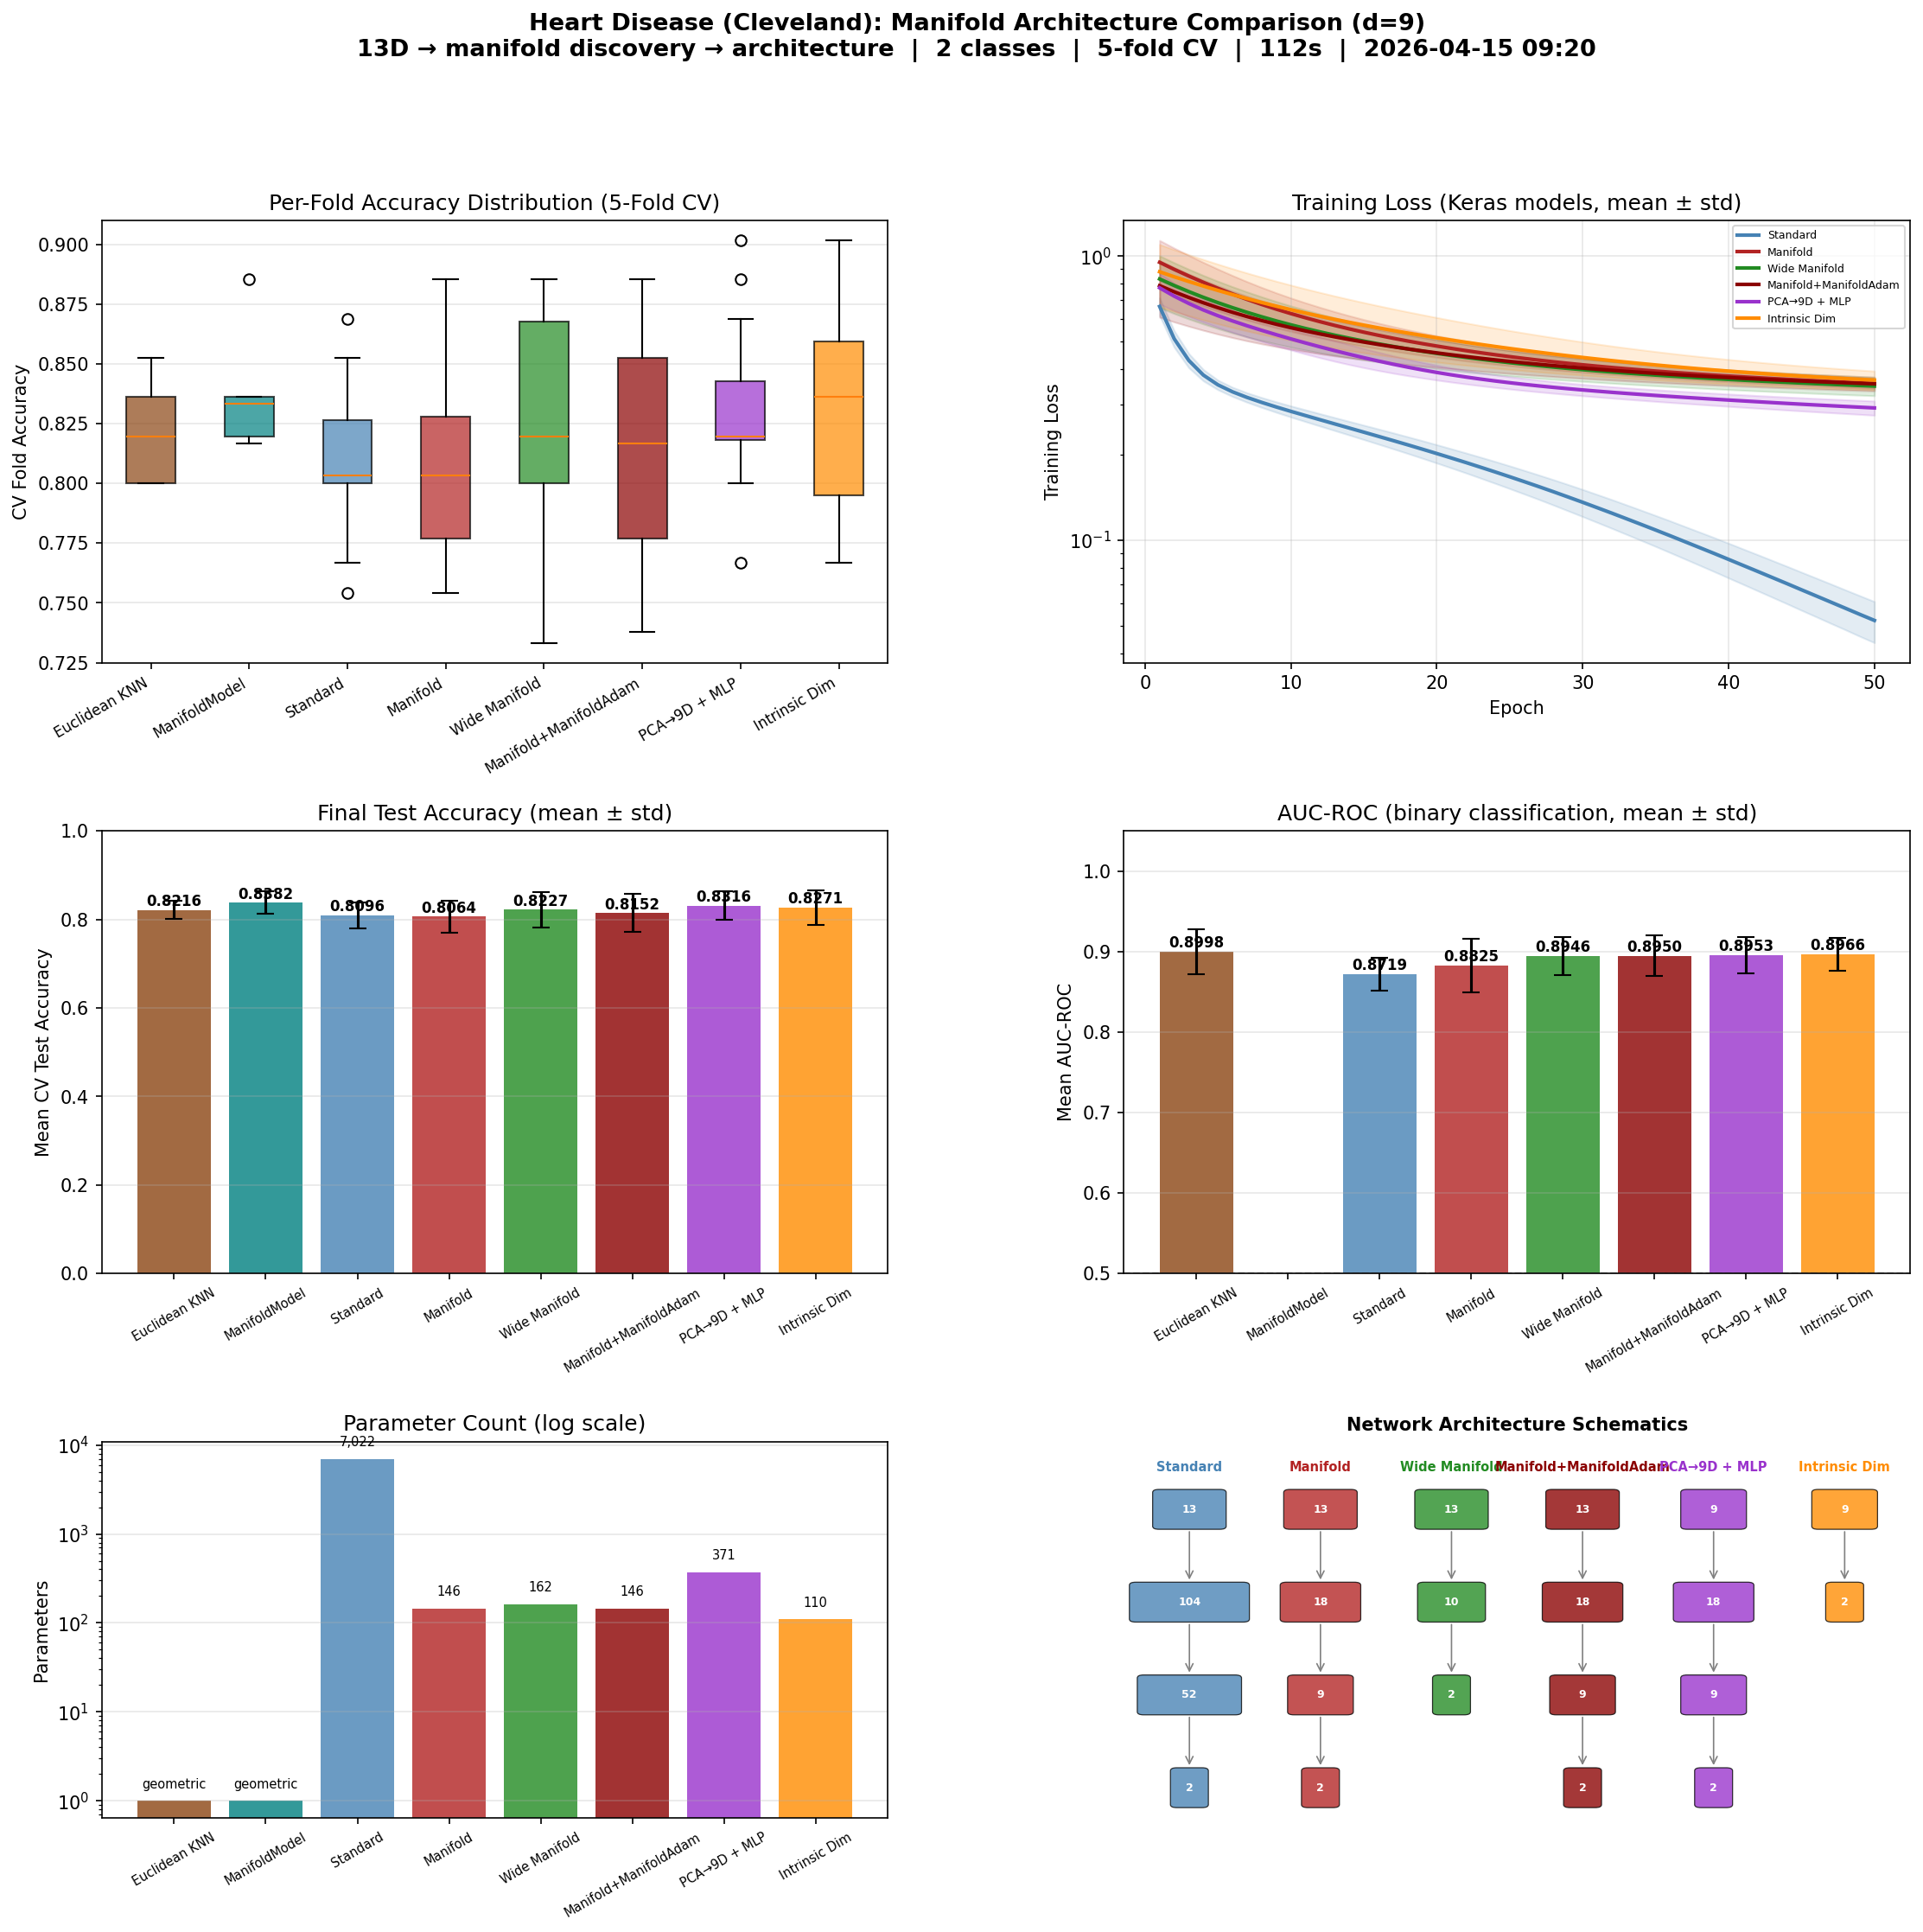
\includegraphics[width=\textwidth]{heart_disease_architecture_results}
\caption{HEART manifold-informed vs.\ standard architecture comparison. $d = 9$, 50 epochs, 3 trials.}
\end{figure}

\section{Provenance}

\begin{tabular}{@{}ll@{}}
\toprule
\textbf{Item} & \textbf{Value} \\
\midrule
  Repository & \href{https://github.com/Flux-Frontiers/waverider}{Flux-Frontiers/waverider} \\
  Commit & \texttt{054030a} (--abbrev-re
054030a600978c0e9ffac58faf7157939927d009) \\
  Commit date & 2026-04-14 22:20:05 -0400 \\
  Commit message & chore(release): bump version to 0.6.0 \\
  Python & 3.12.13 \\
  TensorFlow & 2.21.0 \\
  Device & CPU (forced) \\
  Host & Turing \\
  OS & macOS-26.4-arm64-arm-64bit \\
  Machine & Apple M5 Max MacBook Pro, 64 GB RAM, 2TB SSD \\
  Generated & 2026-04-15 09:41:12 \\
\bottomrule
\end{tabular}

\end{document}
